\documentclass[11pt,a4paper]{article}
\usepackage[T1]{fontenc}
\usepackage[utf8]{inputenc}
\usepackage{newtxtext,newtxmath}
\usepackage[margin=22mm,top=23mm,bottom=23mm,headheight=15pt]{geometry}
\usepackage{microtype}
\usepackage{graphicx}
\usepackage[table]{xcolor}
\usepackage{booktabs,tabularx,array,longtable}
\usepackage{enumitem}
\usepackage{amsmath}
\usepackage{fancyhdr,lastpage}
\usepackage{titlesec}
\usepackage{tcolorbox}
\usepackage{listings}
\usepackage{xurl}
\usepackage{hyperref}
\usepackage{tikz}
\usetikzlibrary{arrows.meta,positioning,fit}
\definecolor{ink}{HTML}{172D42}
\definecolor{teal}{HTML}{087E8B}
\definecolor{pale}{HTML}{EDF5F6}
\definecolor{muted}{HTML}{526674}
\definecolor{line}{HTML}{CBD9DF}
\hypersetup{colorlinks=true,linkcolor=ink,urlcolor=teal,citecolor=teal,
  pdftitle={From Transformer RTL to an Inference Product},
  pdfauthor={Engineering roadmap for the verilog project},
  pdfsubject={Model portability, numerical verification, architecture, ASIC implementation and product delivery}}
\pagestyle{fancy}
\fancyhf{}
\fancyhead[L]{\small\sffamily\color{muted}INFERENCE CHIP / ENGINEERING ROADMAP}
\fancyhead[R]{\small\sffamily\color{muted}21 SEPTEMBER 2026}
\fancyfoot[L]{\small\sffamily\color{muted}Project snapshot and implementation plan}
\fancyfoot[R]{\small\sffamily\thepage\ / \pageref*{LastPage}}
\renewcommand{\headrulewidth}{0.4pt}
\renewcommand{\footrulewidth}{0pt}
\titleformat{\section}{\Large\sffamily\bfseries\color{ink}}{\thesection}{0.65em}{}
\titleformat{\subsection}{\normalsize\sffamily\bfseries\color{ink}}{}{0em}{}
\titlespacing*{\section}{0pt}{0pt}{12pt}
\titlespacing*{\subsection}{0pt}{11pt}{5pt}
\setlength{\parindent}{0pt}
\setlength{\parskip}{6pt}
\setlength{\emergencystretch}{2em}
\setlength{\tabcolsep}{5pt}
\renewcommand{\arraystretch}{1.22}
\setlist[itemize]{leftmargin=1.3em,itemsep=3pt,topsep=4pt,parsep=0pt}
\setlist[enumerate]{leftmargin=1.55em,itemsep=4pt,topsep=4pt,parsep=0pt}
\newlist{checklist}{itemize}{1}
\setlist[checklist]{label=$\square$,leftmargin=1.3em,itemsep=4pt,topsep=4pt}
\newcolumntype{Y}{>{\raggedright\arraybackslash}X}
\BeforeBeginEnvironment{tabularx}{\par\noindent}
\AfterEndEnvironment{tabularx}{\par}
\newcommand{\code}[1]{\texttt{\detokenize{#1}}}
\newcommand{\phase}[2]{\clearpage\section{#1}\label{#2}}
\newcommand{\deliver}[2]{\begin{tcolorbox}[colback=pale,colframe=line,boxrule=0.5pt,arc=1mm,left=8pt,right=8pt,top=6pt,bottom=6pt]\textbf{Deliverable:} #1\par\textbf{Completion evidence:} #2\end{tcolorbox}}
\newcommand{\note}[1]{\begin{tcolorbox}[colback=pale,colframe=teal,boxrule=0.6pt,arc=1mm,left=8pt,right=8pt,top=6pt,bottom=6pt]#1\end{tcolorbox}}
\lstset{basicstyle=\small\ttfamily,backgroundcolor=\color{pale},frame=single,
  rulecolor=\color{line},breaklines=true,columns=fullflexible,keepspaces=true,
  showstringspaces=false,xleftmargin=4pt,xrightmargin=4pt,framesep=6pt}
\begin{document}
\hypersetup{pageanchor=false}
\begin{titlepage}
\thispagestyle{empty}
{\sffamily\color{teal}\large ENGINEERING HANDBOOK\par}
\vspace{20mm}
{\sffamily\bfseries\color{ink}\fontsize{34}{39}\selectfont From Transformer RTL\\to an Inference Product\par}
\vspace{8mm}
{\Large A practical implementation roadmap for real models,\\reusable hardware, and manufactured silicon\par}
\vspace{14mm}
\begin{tcolorbox}[colback=pale,colframe=line,boxrule=0.5pt,arc=1mm]
\textbf{Starting point}\par
The local \code{verilog} project contains a frozen-weight Q8 tile, a CPU reference,
and a small RTL decoder prototype. This handbook identifies what is missing,
what to implement, what to purchase or obtain, and what evidence is required
before claiming a working product.
\end{tcolorbox}
\vspace{8mm}
\textbf{The execution requirement}\par
All transformer forward-pass tensors must be computed by the accelerator.
Host software may prepare models, tokenize text, manage requests, and independently
verify outputs. A CPU numerical result must not silently substitute for missing
hardware inference.
\vfill
{\sffamily\color{ink}\textbf{Version 1.0}\quad 21 September 2026\par}
\vspace{3mm}
{\small Repository: \code{/Users/computer/dev/verilog}\par
Scope: inference only; fixed-model and programmable ASIC choices; large-model scaling.\par
Status: planning document, not a tapeout package or a fabrication quotation.}
\end{titlepage}
\setcounter{page}{2}
\hypersetup{pageanchor=true}

\section*{How to use this handbook}
Start with Sections~\ref{sec:status}--\ref{sec:contract}. They define the actual
starting point and prevent the project from expanding into an undefined promise
to run every possible model. Then work through the implementation gates in
Section~\ref{sec:order}. The checklists describe work packages, not features that
already exist.

\note{\textbf{Recommended direction for your stated goal:} use reloadable weights,
a programmable execution schedule, and a declared operator set. Develop the
correctness and memory interfaces first. Treat a permanently fused model as a
separate specialization after the model and its commercial lifetime are known.}

\subsection*{Read the status labels literally}
\begin{tabularx}{\linewidth}{@{}p{31mm}Y@{}}
\toprule
\textbf{Label} & \textbf{What it establishes}\\\midrule
Implemented prototype & Source exists and some behavior is exercised; correctness or scale may remain unqualified.\\
Verified component & Defined tests or proofs pass for a stated configuration and numerical contract.\\
Mapped hardware & Arithmetic and memories have been implemented using actual target resources.\\
Physical sign-off & Required geometry, connectivity, timing and electrical checks pass for the target flow.\\
Product qualified & Packaged hardware, software, manufacturing test and required qualification have passed.\\\bottomrule
\end{tabularx}

\subsection*{Three rules for reading the estimates}
\begin{enumerate}
\item Capacity and bandwidth examples are calculations with stated assumptions;
they are not measured performance predictions.
\item An arbitrary Verilog array does not establish a feasible physical memory.
Its ports, access latency, banking and electrical behavior must match a real implementation.
\item No finite chip supports arbitrary future architectures. Publish supported
operators, numerical formats, shapes and capacity limits, then reject unsupported models.
\end{enumerate}

\subsection*{Scope and evidence}
The repository observations refer to the files present on 21 September 2026.
Previously recorded experiments are identified as such; this document does not
claim a new full-model inference or physical-design run. External references are
collected at the end. Foundry, supplier, licensing and regulatory details must be
confirmed for the product actually selected.

\clearpage
\begingroup
\small
\setlength{\parskip}{0pt}
\tableofcontents
\endgroup

\phase{Current project: what works and what is still unproven}{sec:status}
\begin{tabularx}{\linewidth}{@{}p{42mm}Y@{}}
\toprule\textbf{Asset} & \textbf{Actual scope}\\\midrule
Frozen model image & Local Llama 3.2 1B Instruct Q8\_0/F32 tensor package: 1,313,251,456 bytes including alignment. It is a data image, not a complete chip.\\
Fixed-weight Q8 tile & Default co-simulation selects eight rows of the first query projection. The physical experiment uses one row. Neither executes a whole attention layer.\\
CPU reference & Complete reference execution; the hybrid path replaces selected CPU outputs with simulated tile outputs. It is not standalone accelerator inference.\\
New decoder RTL & Serial Q16.16 prototype containing the Llama-style graph, mutable parameter arrays, KV state, tied output projection and greedy argmax.\\
Decoder regression & Two layers, hidden width four, two heads, four vocabulary entries and two cached positions; synthetic weights and identity RoPE.\\
Decoder synthesis target & Generic lowering and structural checks; memories and arithmetic operators remain. No target-library timing or completed full gate mapping is established.\\
SKY130 experiment & A separate one-row tile reached placement/clock/global-route stages; no clean final routed implementation of the full decoder.\\\bottomrule
\end{tabularx}

\subsection*{Do not carry these assumptions into a product plan}
\begin{itemize}
\item A test that returns two expected token IDs does not verify every projection,
normalization, probability, activation, or final logit.
\item Increasing elaboration parameters does not prove memory capacity, routing,
clock frequency or runtime model compatibility.
\item Structural synthesis is not equivalent to a clean standard-cell netlist,
physical sign-off, or a working fabricated chip.
\item The older hardmax/ReLU tiny transformer and simulation-only GPT reference
are different designs; their capabilities do not automatically belong to the new decoder.
\end{itemize}
\deliver{A baseline evidence register identifying source revision, model hash,
tool versions, tests and reports for each claim.}{Every status claim links to a
reproducible artifact and lists its configuration and limits.}

\phase{Choose the product and the model-update strategy}{sec:product}
\begin{tabularx}{\linewidth}{@{}p{30mm}Y Y@{}}
\toprule\textbf{Architecture} & \textbf{Strength} & \textbf{Constraint}\\\midrule
Fixed-model ASIC & Specializes weight storage and computation for a chosen checkpoint. & New base weights generally require different manufactured ROM/silicon; adapters only help if supported.\\
Programmable ASIC & Loads new weights and schedules supported operators on the same device. & Pays for writable memory, addressing, control and generality.\\
Hybrid & Combines fixed regions with programmable engines or writable overlays. & Only the deliberately implemented update path is available.\\\bottomrule
\end{tabularx}
Taalas publicly describes specialization for individual models and integration
of storage with computation~\cite{taalas}. Its exact implementation is not a
public specification for this project. Do not assume that an ordinary synthesized
ROM reproduces its physical density or performance.

\subsection*{Write a product requirements document}
\begin{checklist}
\item Select a card, embedded module, appliance, or hosted service as the first deliverable.
\item Identify initial checkpoints and supported architecture variants, including rights to use their weights.
\item Set maximum parameters, layers, hidden/FFN widths, head counts, vocabulary and context.
\item Set batch/concurrency limits, prompt/output length distributions and quality targets.
\item Set time-to-first-token, inter-token latency and throughput targets, including p95/p99 behavior where relevant.
\item Set board power, thermal envelope, dimensions, environmental conditions and host-interface requirements.
\item Set unit-cost target, volume assumptions, support lifetime and model-update policy.
\item Name the reference systems and workloads used to decide whether the product is competitive.
\end{checklist}
Training and optimizer hardware are outside the initial scope. Loading weights
trained elsewhere is sufficient for inference. Supporting adapters or fine-tuning
does not require putting training on this accelerator.
\deliver{Product requirements, a supported-model matrix and an architecture
decision record.}{The first release has measurable limits; model updates and
unsupported operators have explicit behavior.}

\phase{Define the execution and numerical contract}{sec:contract}
The hardware and compiler must agree on exact tensor layouts, data formats,
operation semantics and error behavior. A model name or an ``INT8'' label is
not enough to establish compatibility.
\begin{checklist}
\item Define weight, activation, accumulator and KV formats separately: signedness,
scale/exponent representation, group size, packing, endianness and alignment.
\item Define scale/zero-point interpretation and support for mixed-precision tensors.
\item Specify reduction order, intermediate widths, rounding, saturation, overflow
and underflow; include FP special values wherever FP arithmetic is supported.
\item Define supported shapes, tail masks, strides, transposes, broadcast rules and address widths.
\item Specify nonlinear approximation domains, maximum error and out-of-domain behavior.
\item Set normalization/Softmax precision independently of low-bit matrix weights.
\item Define legal command sequences, reset/cancel behavior, model lifetime and cache validity.
\item State which outputs the accelerator returns: logits, selected tokens, diagnostic tensors, or a supported combination.
\end{checklist}
\subsection*{Separate four meanings of ``exact''}
\begin{tabularx}{\linewidth}{@{}p{34mm}Y@{}}
\toprule\textbf{Property} & \textbf{Evidence needed}\\\midrule
Graph equivalence & Same mathematical operators, dimensions, masks, positions and dependencies as the checkpoint.\\
Arithmetic equivalence & Same specified finite-precision operations and rounding as the chosen hardware oracle.\\
Checkpoint quality & Measured numerical and task-quality impact of quantization and approximation.\\
Product reliability & Correct execution under supported workloads, stalls, resets and operating conditions.\\\bottomrule
\end{tabularx}
A lower-precision implementation can preserve the graph while producing
different logits. An approximate exponential is not automatically acceptable
because it is synthesizable. Choose tolerances before evaluating results.
\deliver{A numerical specification and operator/interface conformance suite.}{Two
independent implementations agree within the specified contract, including edge cases.}

\phase{Repair and qualify the current arithmetic and protocols}{sec:repairs}
Treat these as priority engineering tasks before adding larger matrices.
\begin{tabularx}{\linewidth}{@{}p{38mm}Y@{}}
\toprule\textbf{Current issue} & \textbf{Required action and test}\\\midrule
Q16.16 resolution & Its LSB is $2^{-16}\approx1.526\times10^{-5}$. Select a representation for the checkpoint's $10^{-5}$ RMS epsilon and qualify the resulting error.\\
Exponential clipping & The current function clips to $[-8,8]$. Measure probability-tail and SiLU errors; replace it with a bounded-error implementation for the actual domain.\\
Softmax range & A Q16.16 sum saturates near 32,768 unit exponentials. Widen/rescale accumulators and prove supported context limits.\\
Premature saturation & Per-product/per-add saturation can destroy cancellation. Use justified accumulator width and test long mixed-sign reductions.\\
Signed arithmetic & Audit signed division, negation of the most-negative integer, casts and concatenations. Test positive/negative operands against an independent oracle.\\
Unpipelined operators & Division, square root and dependent multipliers need implementation latencies and timing constraints; source-level operators alone are insufficient.\\
Input lifetime & Latch token/command inputs when accepted or define and verify a stable-input contract. The present embedding reads the token over multiple cycles.\\
Context/model changes & Report full-context and invalid-token errors. Block incompatible model writes or invalidate KV state; define clear/start priority.\\
Small regression & Add nonidentity RoPE, signed/random tensors, intermediate checks and full-cache/reset/stall cases.\\\bottomrule
\end{tabularx}
The current test exercises some nonzero arithmetic, but it mainly checks argmax,
position and positivity. It does not establish full numeric correctness. No
repairs to RTL are performed by producing this handbook.
\deliver{A reviewed issue list, arithmetic units with a defined contract, and
regression vectors.}{All listed behaviors have passing tests; unsupported ranges
produce defined errors rather than silent wrong results.}

\phase{Build the model importer and compiler}{sec:compiler}
The importer translates a checkpoint into the accelerator's representation. The
compiler maps its graph onto available compute and memory resources.
\begin{checklist}
\item Parse supported containers and configuration metadata; validate tensor count,
names, shapes, data types and file bounds before allocation or execution.
\item Handle tied/separate embedding and output weights, biases, norm constants,
head grouping, tensor permutations and RoPE conventions.
\item Decode supported quantization formats. Q8\_0 consists of an FP16 block scale
and 32 signed INT8 values; other ``8-bit'' formats are not necessarily interchangeable.
\item Define whether to preserve Q8\_0 or calibrate a new format. Expanding a
previously quantized checkpoint does not recover its original lost precision.
\item Pack weights, scales and constants into aligned banks; generate bank addresses
and integrity hashes without silently dropping unsupported tensors.
\item Allocate activation/residual lifetimes, scratch space and KV storage.
\item Tile and fuse supported operations; schedule memory transfers, reductions and barriers.
\item Emit instructions/descriptors plus a manifest containing dimensions, operator
requirements, numerical contract, compiler version and model hash.
\item Validate capacity and address calculations using widths large enough for the
largest image; do not rely on signed 32-bit host/RTL intermediates for huge tensors.
\item Provide explicit diagnostics for unsupported operations, formats or capacity.
\end{checklist}
\subsection*{Offline software is compatible with hardware inference}
Python or C++ may prepare constants, including a qualified RoPE lookup table,
and independently compute expected results. During an inference run, all
transformer tensors must come from the hardware datapath. The runtime must not
quietly route unsupported transformer operations to the CPU.
\deliver{Importer, compiler, model-image format, loader compatibility rules and
test corpus.}{A real checkpoint imports reproducibly; its generated schedule
executes without host tensor substitution.}

\phase{Implement reusable matrix and vector engines}{sec:compute}
\subsection*{Matrix engine}
\begin{checklist}
\item Implement GEMV for incremental decode and GEMM for prompt processing/batching.
\item Select lane count, multiplier precision, accumulator width, pipeline depth
and reduction topology from bandwidth, area and performance budgets.
\item Support programmable dimensions, strides, base addresses and matrix tiling.
\item Handle partial tiles, ragged dimensions, transposes and masked tail lanes.
\item Accept mutable activation operands for attention, not only fixed weight operands.
\item Implement weight unpacking, block scales, quantization/dequantization and output conversion.
\item Provide banked accumulators, input/output buffers and overlap of transfer with computation.
\item Export completion, exceptions, utilization and stall counters.
\end{checklist}
\subsection*{Vector and reduction engine}
\begin{checklist}
\item Implement add, multiply, bias, sum, maximum and sum-of-squares reductions.
\item Implement RMSNorm; add LayerNorm only if included in the declared model set.
\item Implement reciprocal/reciprocal-square-root, exponential, SiLU and any required GELU variant.
\item Implement residuals, quantization, clipping and model-specific logit transforms where required.
\item Give every multicycle unit an explicit request/response protocol and reset behavior.
\item Size shared resources so normalization and Softmax do not stall a much larger matrix array indefinitely.
\end{checklist}
An RTL function call can instantiate substantial combinational hardware at each
call site. Serial control does not automatically mean that synthesis shares a
single physical arithmetic unit. Inspect the mapped structure and resource use.
\deliver{Parameterized compute engines with latency-aware interfaces and a mapped
representative tile.}{Operator accuracy, stall behavior, resource use and timing
are measured for the selected target.}

\phase{Complete the transformer graph and attention}{sec:attention}
For the Llama-style path, the per-token computation is:
\begin{align*}
n &= \operatorname{RMSNorm}(x), & Q&=W_Qn,\quad K=W_Kn,\quad V=W_Vn,\\
\widehat Q&=\operatorname{RoPE}(Q), &\widehat K&=\operatorname{RoPE}(K),\\
P&=\operatorname{softmax}\!\left(\frac{\widehat Q K_{\rm cache}^{T}}{\sqrt{d_h}}+M\right),
&r&=x+W_O(PV_{\rm cache}),\\
u&=\operatorname{RMSNorm}(r), & y&=r+W_{\rm down}\bigl[\operatorname{SiLU}(W_{\rm gate}u)\odot W_{\rm up}u\bigr].
\end{align*}
The current token's rotated K and V must be appended before its attention reads
them. $M$ denotes the applicable mask; GQA maps query heads onto their shared KV
heads. Norm weight vectors and epsilon are part of each normalization.
\begin{checklist}
\item Verify all Q/K/V/O dimensions and head permutations against checkpoint conventions.
\item Support required position indices, rotary dimensions, frequencies and scaling.
\item Implement the appropriate causal, padding and optional sliding-window masks.
\item Compute QK scores, stable Softmax and probability-weighted V in the specified precision.
\item Implement prompt and decode execution modes with consistent cache contents.
\item Consider streaming/tiled Softmax to reduce attention intermediate storage;
qualify its accumulation order and approximation error.
\item Preserve residuals until consumed and schedule all layers without CPU math.
\item Execute embedding lookup, final normalization and vocabulary projection.
\item Support untied output weights where required; the present prototype assumes tied weights.
\end{checklist}
The prefill score domain grows with prompt length; incremental decode reads an
existing cache. Their data reuse and scheduling differ. NVIDIA's documentation
provides concrete examples of attention and cache-serving modes~\cite{attention}.
\deliver{One full real-checkpoint layer, then the complete real decoder.}{Compare
intermediate tensors and final logits across multiple tokens and nontrivial positions.}

\phase{Engineer weight memory, scratchpads and data movement}{sec:memory}
\begin{checklist}
\item Budget weight bytes, scales, padding, protection, activations, residuals,
accumulators, instructions and KV separately.
\item Choose on-chip ROM/SRAM capacity and any external memory technology based on
both sustainable bandwidth and storage demand.
\item Define banks, ports, access width, latency, burst length and alignment.
\item Obtain usable memory macro views: functional model, timing, physical abstract,
layout, power and electrical information required by the flow.
\item Implement a memory controller and its PHY for external DRAM, including
initialization, training/calibration, refresh and error reporting as applicable.
\item Implement DMA, queues, arbitration, response tracking and backpressure.
\item Double-buffer transfers where useful and budget all in-flight data.
\item Provide scale/metadata bandwidth alongside weight bandwidth.
\item Define read/write collision behavior and map it to the selected macros.
\item Add appropriate error detection/correction, test, repair or redundancy.
\end{checklist}
\subsection*{A realistic integration boundary}
\begin{center}
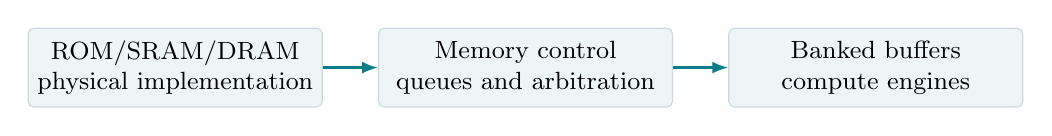
\begin{tikzpicture}[node distance=7mm,box/.style={draw=line,fill=pale,rounded corners=2pt,minimum height=10mm,text width=35mm,align=center,font=\small},arr/.style={-{Latex[length=2mm]},thick,color=teal}]
\node[box] (mem) {ROM/SRAM/DRAM\\physical implementation};
\node[box,right=of mem] (ctrl) {Memory control\\queues and arbitration};
\node[box,right=of ctrl] (buf) {Banked buffers\\compute engines};
\draw[arr] (mem) -- (ctrl);
\draw[arr] (ctrl) -- (buf);
\end{tikzpicture}
\end{center}
The present asynchronous array reads and broad access patterns are not a
complete SRAM interface. A new latency-aware interface is required before
claiming a memory macro can simply replace an array. A full Q16.16 image for
the current 1B model would consume roughly 4.94 GB, before dynamic state.
\deliver{Memory architecture, address map, controller/PHY integration and macro
contracts.}{The complete workload runs with realistic latency, stalls and
capacity limits; no ideal zero-latency memory assumption remains hidden.}

\phase{Size model storage, KV capacity and bandwidth}{sec:sizing}
For $P$ stored parameters at $q$ bits each, bare weight storage is
\[
M_W = \frac{Pq}{8}\quad\text{bytes},
\]
before scales, zero points, alignment, replication, repair and error protection.
\begin{center}
\begin{tabular}{@{}lrr@{}}
\toprule\textbf{Stored parameters} & \textbf{8-bit} & \textbf{4-bit}\\\midrule
1 billion & 1 GB & 0.5 GB\\
8 billion & 8 GB & 4 GB\\
70 billion & 70 GB & 35 GB\\
405 billion & 405 GB & 202.5 GB\\
1 trillion & 1 TB & 500 GB\\\bottomrule
\end{tabular}
\end{center}
These are decimal units and hypothetical precision choices, not a claim that
all checkpoints preserve acceptable quality at four bits.

For conventional MHA/GQA with uniform dimensions and cache precision,
\[
M_{\rm KV}=2BLTH_{\rm KV}D_hb.
\]
$B$ is concurrent sequences, $L$ layers, $T$ cached tokens, $H_{\rm KV}$ KV heads,
$D_h$ head size and $b$ bytes per cached element. The factor two accounts for K and V.
For the local model ($L=16$, $H_{\rm KV}=8$, $D_h=64$), an FP16 cache requires
256 MiB at 8,192 tokens or 4 GiB at 131,072 tokens \emph{per conversation}.
The present 32-bit cache representation doubles those amounts. MLA and recurrent
architectures need different storage equations.

For dense batch-one decode with one full external matrix-weight read per token,
\[
\mathrm{BW}_{W}\gtrsim M_W R,
\]
where $R$ is tokens/s. A hypothetical 70B, 4-bit, 100-token/s target requires
at least 3.5 TB/s for bare weights alone. Its dense projection work is roughly
$2P$ operations/token (multiply and add counted separately), or 14 TOP/s in
the implemented number format, excluding attention and nonlinearities.

Batching can amortize weight reads; local weights change where bandwidth must
be provided. Neither estimate is an achieved rate. Actual latency is bounded
by compute, memory, communication and dependencies, with imperfect overlap.
\deliver{A capacity/bandwidth worksheet for every supported workload.}{Every
claimed rate fits sustainable hardware budgets with explicit utilization and overhead assumptions.}

\phase{Manage KV state, requests and long contexts}{sec:kv}
\begin{checklist}
\item Track request ownership, model identity, sequence length and token position.
\item Define per-layer/head cache layouts and append/read ordering.
\item Check capacity before acceptance; report full-context errors explicitly.
\item Allocate, release and reuse storage without cross-request reads.
\item Invalidate incompatible caches when the model, adapter or relevant execution configuration changes.
\item Define reset, cancel, abort, retry and context-restart behavior.
\item Introduce paging or block allocation if required for long contexts and concurrency.
\item Add eviction/sliding-window behavior only when consistent with the model and product promise.
\item Qualify KV quantization independently of weight quantization.
\item Define ownership/reference counting for shared prefixes if supported.
\item Budget cache read bandwidth as context grows, not just storage bytes.
\item Enforce access isolation and any required erasure policy.
\end{checklist}
\subsection*{Production scheduling}
Continuous batching, chunked prompt processing and admission control can improve
utilization, but add request IDs, synchronization and resource-management logic.
Decide whether prompt and decode work share a device or use separate resources;
the latter also requires KV transfer and coordination.

\note{\textbf{Current cache behavior:} \code{clear_cache} resets the valid position;
it does not overwrite every KV bit. Logical invalidation can support dense SRAM
mapping, but it is not physical data erasure. The integration must prevent stale
entries from being read or exposed.}

\deliver{Cache manager, allocation policy and request-lifecycle specification.}{Tests
cover full capacity, reuse, model changes, cancellations, multiple users and
long-context numerical behavior with no stale or cross-request state.}

\phase{Make execution programmable and observable}{sec:control}
Changing RTL parameters changes elaborated hardware. Runtime model portability
requires a supported instruction set, descriptors or microcode plus reloadable weights.
\begin{tabularx}{\linewidth}{@{}p{37mm}Y@{}}
\toprule\textbf{Descriptor field} & \textbf{Required meaning}\\\midrule
Opcode and version & Supported operation and compatible command format.\\
Tensor references & Source/destination bases, dimensions, strides and bounds.\\
Numerics & Formats, scale locations, accumulation and output rules.\\
Dependencies & Ordering, barriers, events and buffer lifetime.\\
Request identity & Model/context ownership and completion destination.\\
Status & Completion, error reason, progress and performance counters.\\\bottomrule
\end{tabularx}
\begin{checklist}
\item Latch accepted commands; use explicit ready/valid or equivalent handshakes.
\item Check opcodes, formats, addresses and dimensions before issuing accesses.
\item Define backpressure, queue depth, outstanding operations and completion ordering.
\item Provide timeouts, watchdogs, cancellation and recovery from invalid state.
\item Define priorities for simultaneous reset, cache clear, configuration and start.
\item Protect model loading against inference using partially written parameters.
\item Expose model/firmware IDs, cycle counts, bytes moved, engine utilization and stall reasons.
\item Add limited trace or diagnostic readback to locate the first incorrect tensor.
\item Provide output backpressure or a documented bounded-buffer protocol.
\end{checklist}
A hardware sequencer may be an FSM, microcoded controller, or management CPU
issuing accelerator commands. The constraint is that the accelerator computes
the transformer tensors; it does not prohibit software that schedules operations.
\deliver{Command/register specification, sequencer, trace facilities and conformance
tests.}{Legal programs execute correctly under stalls; invalid requests fail
predictably without corrupting another request.}

\phase{Support different families and very large models}{sec:portability}
\begin{tabularx}{\linewidth}{@{}p{36mm}Y@{}}
\toprule\textbf{Model feature} & \textbf{Additional support to plan}\\\midrule
GPT-style variants & LayerNorm, biases, GELU variants, learned or alternative positions.\\
Attention variants & MHA/MQA/GQA layout rules, masks, windows, position scaling and separate output weights.\\
Mixture of experts & Router/top-k selection, token dispatch, expert addressing, imbalance handling and weighted output combination.\\
Latent attention & Its projection graph and compressed cache representation.\\
Encoder--decoder & Encoder computation, cross-attention and encoder-state storage.\\
Vision/audio & Required frontend operators, preprocessing, encoder and cross-modal integration.\\
Recurrent/state-space & Architecture-specific state updates, scans, convolution or other operators.\\
Adapters & Storage, low-rank projections, selection, model/cache compatibility and quality tests.\\\bottomrule
\end{tabularx}
The support matrix must specify subsets rather than promise all of these at once.
DeepSeek-V3, for example, documents 671B total parameters, 37B active per token,
MoE and MLA~\cite{deepseek}. A dense Llama loop with larger parameters does not
implement that graph. Active parameters reduce some work per token; total expert
weights still require a storage strategy.

\subsection*{Beyond a single chip}
\begin{checklist}
\item Select tensor, pipeline and/or expert parallelism; generate partitions in the compiler.
\item Budget link latency/bandwidth and collectives: reductions, gathers and routed expert traffic.
\item Implement physical links, packet queues, flow control, synchronization and integrity checks.
\item Define topology, retry/failure behavior and deadlock prevention.
\item Coordinate distributed model loading, request state, completion and recovery.
\item Budget package/board/rack power, cooling and network capacity at the system level.
\end{checklist}
\deliver{A bounded compatibility matrix and, if needed, a multi-device execution
design.}{A second supported model runs on unchanged hardware; a partitioned
model matches its single-system reference and survives communication stalls.}

\phase{Build independent verification and release evidence}{sec:verification}
Verification should expose incorrect arithmetic and incorrect dataflow, not
merely demonstrate that the controller eventually asserts \code{done}.
\begin{checklist}
\item Establish an independent oracle with specified arithmetic semantics and real checkpoint data.
\item Test signed extrema, zeros, tiny values, scale outliers, rounding ties and long reductions.
\item Compare Q/K/V projections, norm statistics, RoPE outputs, attention scores,
probabilities, FFN intermediates and final logits.
\item Test nonidentity rotary angles and long-context position behavior.
\item Exercise nonmultiple tiles, supported shape boundaries and overflow in address calculations.
\item Inject memory stalls, variable latency, backpressure and interruptions.
\item Test reset/cancel mid-operation, full-cache behavior, model updates and request isolation.
\item Add assertions for valid state transitions, bounds, ordering and completion.
\item Use code/functional coverage and review uncovered behaviors; coverage percentage alone is not correctness.
\item Use formal properties for suitable blocks/protocols and equivalence checks across synthesis/ECO steps.
\item Run gate-level and timing-aware checks appropriate to the design and tool flow.
\item Evaluate model quality over multiple prompts, tasks and context lengths; matching one answer is insufficient.
\end{checklist}
\subsection*{Preserve a reproducible evidence bundle}
Store source revision, model hash, numerical contract, generator seed, tool and
IP versions, configuration, expected/observed values, tolerances, logs and result
summary. Make regressions run automatically when RTL, compiler, firmware or model
packing changes. Record approved exceptions with owner and rationale.
\deliver{Operator, layer, model, protocol and implementation regression suites.}{A
release candidate meets declared quality limits and all required checks; numerical
and hardware failures identify a reproducible first point of divergence.}

\phase{Model performance and validate on a hardware prototype}{sec:performance}
Measure prompt processing and generation separately. A high peak MAC count can
coexist with poor token latency if memory, reductions or communication starve it.
\begin{checklist}
\item Build a cycle/data-movement model with actual memory ports, transfer sizes,
queue depth, dependencies and clock assumptions.
\item Estimate area and power from representative mapped blocks and memory macros.
\item Measure prefill latency, time to first token, decode latency and aggregate throughput.
\item Sweep prompt length, generated length, batch size and request concurrency.
\item Record p95/p99 latency and admission/queue behavior where relevant.
\item Profile bank conflicts, stalls, arithmetic utilization and bytes transferred.
\item Measure chip/card/system power at clearly stated boundaries; calculate energy per token.
\item Compare model quality at the same numerical settings used for speed measurements.
\item Use an FPGA/emulation prototype with real memory traffic to validate integration.
\item Separate prototype clock/resource limits from target ASIC projections.
\end{checklist}
\subsection*{Minimum benchmark record}
\begin{tabularx}{\linewidth}{@{}p{38mm}Y@{}}
\toprule\textbf{Record} & \textbf{Required context}\\\midrule
Model and software & Checkpoint hash, compiler/runtime version, precision and quality result.\\
Workload & Prompt/output lengths, context, sampling policy, concurrency and warm/cold state.\\
Hardware & Devices, memory, clocks, cooling and measurement method.\\
Performance & First-token latency, inter-token latency, throughput, variability and repetitions.\\
Energy/cost & Power boundary, energy per token, utilization and cost assumptions.\\\bottomrule
\end{tabularx}
MLPerf provides a reference for defined inference workloads and quality
requirements~\cite{mlperf}. Do not claim formal benchmark compliance without
following the applicable rules.
\deliver{A measured prototype report and revised capacity/area/power budget.}{The
claimed workload meets its targets with no hidden host tensor computation or
unreported precision/quality change.}

\phase{Integrate the chip platform and obtain technology IP}{sec:soc}
\subsection*{Digital platform}
\begin{checklist}
\item Select host transport, register map, DMA, command queues and interrupts.
\item Integrate boot/configuration control and firmware storage where needed.
\item Design clock/reset distribution and verify clock-domain/reset-domain crossings.
\item Add clock gating, power management and valid power-state transitions.
\item Provide watchdogs, debug access, performance counters and error reporting.
\item Add temperature/voltage monitoring and controlled thermal throttling where required.
\item Protect host/DMA address ranges and isolate requests appropriate to the deployment.
\item Define model/firmware integrity, update and rollback requirements.
\end{checklist}
\subsection*{Foundry and licensed implementation inputs}
\begin{checklist}
\item Select foundry, process, approved design kit, standard cells and sign-off flow.
\item Obtain SRAM/ROM macros with the required size, banking, ports and characterized corners.
\item Obtain I/O, ESD, level-shifter/isolation and power-domain cells as needed.
\item Obtain clock-generation IP if the chip needs an internal PLL/oscillator.
\item Obtain memory controller/PHY and high-speed interface IP for selected external interfaces.
\item Confirm physical, timing, electrical, functional and test views are mutually compatible.
\item Resolve license/manufacturing rights, support, integration constraints and package requirements.
\end{checklist}
Do not equate an open PDK installation with an agreed commercial production
flow. The public SKY130 documentation describes the status and limitations of
its release~\cite{sky130}; confirm accepted tools, decks and qualification with
the actual fabrication partner. A process node alone does not establish that
the required memory or interface IP is available.
\deliver{System specification, IP inventory, technology agreement and integration
models.}{All hard macros and interfaces have usable views, verified integration
and a path accepted by the fabrication partner.}

\phase{Close physical design and prepare a tapeout package}{sec:physical}
\begin{checklist}
\item Establish floorplan, hierarchy, macro placement, pin/bump constraints and routing channels.
\item Design the power grid using estimated current, package delivery and decoupling needs.
\item Write complete clock, I/O, uncertainty, load and timing-exception constraints.
\item Map logic to the chosen libraries; insert appropriate test and power structures.
\item Place cells, construct clock trees and complete detailed routing.
\item Extract parasitics and close setup/hold timing across required modes and corners.
\item Check clock quality, unconstrained paths, signal integrity and crosstalk as applicable.
\item Analyze static/dynamic voltage drop and electromigration with justified activity assumptions.
\item Complete DRC, LVS, electrical, antenna, density and manufacturing-rule checks.
\item Add required fill, seal ring, die identification, pads/bumps and package connectivity.
\item Recheck equivalence and timing after engineering changes.
\item Release GDS/OASIS and required netlists, abstracts, constraints, reports and checksums.
\end{checklist}
\subsection*{Define acceptable closure with the foundry}
The goal is no unapproved violations under the selected sign-off rules. Any
waiver must be reviewed and accepted by the responsible design/fabrication
authority; a script returning successfully is not an engineering waiver.

The older one-row SKY130 experiment does not predict full-decoder area by a
simple multiplier. Memory topology, cell implementation, routing and clock
distribution change with architecture. Nor does the new generic structural
target establish the absence of combinational mapping problems.
\deliver{A reviewed tapeout package and signed release checklist.}{The exact
released design passes required checks, uses accepted IP views and matches the
package/manufacturing submission rules.}

\phase{Design production test and silicon reliability}{sec:test}
\begin{checklist}
\item Develop a design-for-test plan before physical implementation is finalized.
\item Insert scan/test access and generate automated fault patterns as appropriate.
\item Cover stuck-at and timing-related faults with measurable targets and justified exclusions.
\item Add SRAM self-test, repair/redundancy and ROM verification where supported.
\item Plan boundary scan, test clocks, reset control and power modes.
\item Create wafer-probe and packaged-part test flows, fixtures and program versions.
\item Define pass/fail bins, test limits, test time and traceability requirements.
\item Characterize voltage/frequency/temperature operating margins.
\item Qualify ESD, latch-up, package integrity and lifetime behavior for the target market.
\item Plan fault injection, field error reporting and recoverable failure behavior.
\item Establish yield analysis, failure analysis and a feedback process for revisions.
\end{checklist}
\subsection*{First-silicon bring-up order}
\begin{enumerate}
\item Verify rails, current draw, clock and reset using safe initial conditions.
\item Establish debug/register access and identify chip/firmware versions.
\item Exercise SRAM, ROM and external-memory initialization/test.
\item Check arithmetic units and small known tensor transfers.
\item Run a known layer, then a full model, against stored reference outputs.
\item Sweep workloads, clocks, voltage/temperature conditions and interfaces within approved limits.
\end{enumerate}
Manufacturing yield and reliability are separate from neural-network numerical
quality. A design must satisfy both, with a test policy that can distinguish
silicon defects from software or model-image failures.
\deliver{DFT architecture, test patterns/programs, characterization and qualification
plan.}{Working parts can be identified repeatably, faulty parts rejected and field
failures traced to a reproducible configuration.}

\phase{Build the package, board, cooling and service software}{sec:board}
\subsection*{Physical product}
\begin{checklist}
\item Select package technology, substrate, pin/bump assignment and escape routing.
\item Co-design power/ground delivery, signal routing and thermal paths.
\item Create PCB schematics, stack-up, impedance constraints and layout.
\item Specify regulators, rail sequencing, protection, decoupling and clock sources.
\item Route external memory and host interfaces with signal/power integrity checks.
\item Provide debug/programming connectors, sensors, test points and assembly fixtures.
\item Design heatsink, airflow, thermal interface, mounting and enclosure.
\item Release BOM, fabrication/assembly data and board production tests.
\end{checklist}
\subsection*{Software a customer can use}
\begin{checklist}
\item Deliver firmware, driver, model loader and a documented runtime API.
\item Validate model/firmware/compiler compatibility and failure reporting.
\item Provide tokenization, templates and generation controls promised by the product.
\item Decide logits versus token output; argmax supplies greedy decoding only.
\item Implement temperature, top-k/top-p, penalties and RNG if supported; identify
whether sampling runs on host or accelerator.
\item Support request admission, scheduling, cancellation and memory accounting.
\item Deliver installation packages, examples, diagnostics, monitoring and profiling.
\item Establish signed/versioned releases as appropriate, update/rollback procedures and support policy.
\end{checklist}
The host may tokenize and serve requests while the accelerator owns the complete
transformer forward pass. Make that boundary observable in tests and product
documentation so users can distinguish hardware execution from reference software.
\deliver{Packaged device, reference board and installable software release.}{A new
user can install the system, load a supported model, run inference and diagnose
documented errors without developer-only intervention.}

\phase{Resolve commercial, licensing and compliance work}{sec:commercial}
\begin{checklist}
\item Review checkpoint redistribution/commercial terms, notices, branding and permitted uses.
\item Review third-party software, RTL, EDA and hard-IP licenses, including manufacturing rights.
\item Review implementation IP/patent exposure with appropriate specialists.
\item Determine product/export classification, destinations and end-user requirements.
\item Identify applicable EMC, safety and environmental obligations for the final product and markets.
\item Define privacy/data-handling obligations for any hosted service.
\item Establish warranty, returns, support, service-level and liability terms.
\item Secure foundry, assembly/test, memory, board and cooling suppliers with realistic lead times.
\item Plan qualification, production ramps, lot traceability, inventory and revision management.
\end{checklist}
Embedding weights in silicon does not remove their license conditions. Meta's
Llama 3.2 license includes obligations for redistribution/products containing
the materials~\cite{llama-license}. EU manufacturers must identify applicable
legislation and perform the relevant conformity process~\cite{eu}. Advanced
computing export requirements depend on specifications, jurisdiction and
destination; review current rules for the selected product~\cite{bis}.

\subsection*{Fund a shipped product, including revisions}
Obtain quotations for engineering, EDA/compute, memory/interface IP, masks,
prototype runs, wafers, yield, packaging, test, boards, memory, cooling,
qualification and support. Include rework/respin contingency. Distinguish
prototype shuttle cost from production economics.
\begin{align*}
C_{\rm shipped}\approx{}&C_{\rm good\ die}+C_{\rm package/test}
+C_{\rm board/memory/cooling}\\
&+C_{\rm assembly/support}+\frac{C_{\rm development}}{N_{\rm shipped}}.
\end{align*}
Assign owners for architecture, numerics, RTL, verification, physical design,
DFT, compiler/runtime, board design and manufacturing. These roles may be
partners or staff; no universal team size or fabrication price is assumed here.
\deliver{Commercial plan, supplier/IP agreements and compliance responsibility
matrix.}{The product has a viable cost model and a documented route to legal,
repeatable manufacture and sale in its selected markets.}

\phase{Execute the project in evidence-based stages}{sec:order}
\begin{tabularx}{\linewidth}{@{}p{14mm}p{39mm}Y@{}}
\toprule\textbf{Gate} & \textbf{Work package} & \textbf{Exit evidence}\\\midrule
G0 & Freeze scope and baseline & Product limits, model/format choices, source snapshot and claim register.\\
G1 & Arithmetic/protocol repair & Independent signed arithmetic, nonlinear, bounds and handshake regressions.\\
G2 & Real checkpoint layer & Hardware computes norm, QKV, RoPE, cache, attention and FFN with validated intermediate tensors.\\
G3 & Full real model & All layers and final logits execute through hardware across representative prompts and contexts.\\
G4 & Runtime portability & A second supported checkpoint/configuration runs on unchanged hardware using the importer and schedule.\\
G5 & Realistic memory & Same execution succeeds with memory latency, bandwidth, stalls, capacity and error behavior represented.\\
G6 & Performance prototype & Measured quality, throughput, latency and power/resource evidence against product targets.\\
G7 & Multi-device scale, if needed & Correct partitioned execution, communication budget and recovery behavior.\\
G8 & Tapeout readiness & Technology/IP, DFT, mapped design, physical closure and accepted sign-off package.\\
G9 & First silicon & Packaged parts pass bring-up, interfaces, memory, tensor and model tests.\\
G10 & Product release & Qualification, manufacturing test, usable software, support and commercial obligations complete.\\\bottomrule
\end{tabularx}
\subsection*{Start with these concrete actions}
\begin{enumerate}
\item Record the current sources and existing test scope; stop treating the tiny
argmax smoke test as evidence of real-model correctness.
\item Choose a first supported checkpoint, context limit and numerical contract.
Write focused regressions for the arithmetic/protocol risks in Section~\ref{sec:repairs}.
\item Define a latency-aware model-memory interface and a checkpoint packer that matches it.
\item Validate one real layer tensor by tensor, then all layers, then a second model.
\item Obtain representative memory/IP data early and use it to constrain architecture
before committing to expensive physical implementation.
\end{enumerate}
These are dependency gates, not calendar estimates. IP availability, numerical
results and prototype measurements can require architectural revisions.

\phase{Maintain a release checklist and risk register}{sec:release}
\begin{checklist}
\item Supported-model/operator matrix is published and versioned.
\item Trained weights and executable image are hashed and traceable.
\item Quantization and numerical quality meet predeclared thresholds.
\item No CPU tensor result contributes to the advertised hardware forward pass.
\item Real-memory latency/bandwidth and error behavior are represented in verification.
\item Context, shape, address and concurrency limits are enforced.
\item A second model demonstrates portability if portability is advertised.
\item Required timing, equivalence, physical and electrical checks pass.
\item Manufacturing test and qualification meet agreed targets.
\item Package, board, firmware, driver and model loader versions are compatible.
\item Performance claims include workload, quality and measurement boundaries.
\item Suppliers, licenses, compliance owners and support procedures are assigned.
\end{checklist}
\subsection*{Track risks as decisions, not vague concerns}
\begin{tabularx}{\linewidth}{@{}p{30mm}Y Y@{}}
\toprule\textbf{Risk} & \textbf{Early evidence} & \textbf{Possible response}\\\midrule
Numerical quality & Layer/logit error and task evaluation & Revise formats, accumulators or approximations.\\
Memory feasibility & Capacity/ports/area/bandwidth from actual macros & Change banking, capacity, external-memory or partition plan.\\
Timing/congestion & Representative mapped/routed blocks & Pipeline, simplify interfaces, repartition or revise clock target.\\
Poor utilization & Counters and traffic model & Revise dataflow, buffering, batch policy or lane count.\\
Model obsolescence & Update policy and customer workload & Favor reloadable weights or limit fixed-model commitments.\\
Yield/cost & Supplier quotes, test plans and die/package estimates & Revise die size, redundancy, packaging, volume or product target.\\\bottomrule
\end{tabularx}
Give each entry an owner, evidence link, next experiment, decision deadline and
impact on scope. A prototype result should update the plan rather than become
an unsupported product claim.

\phase{Repository map and commands}{sec:repo}
Paths below are relative to \code{/Users/computer/dev/verilog}. They identify the
current prototype, not a promise that every proposed subsystem already exists.
\begin{tabularx}{\linewidth}{@{}p{67mm}Y@{}}
\toprule\textbf{Path} & \textbf{Purpose}\\\midrule
\code{rtl/llama_decode_core.sv} & Serial Q16.16 Llama-style decoder prototype.\\
\code{tb/tb_llama_decode_core.sv} & Tiny two-layer/two-token synthetic smoke test.\\
\code{asic/llama.mk} & Decoder generic-lowering and older frozen-tile targets.\\
\code{asic/llama_frozen_tile_top.sv} & Selected fixed-weight Q8 projection tile.\\
\code{rtl/q8_0_dot_pipeline.sv} & Pipelined signed block-dot arithmetic for the frozen tile.\\
\code{tools/freeze_llama.py} & Frozen image/selected-tile preparation.\\
\code{tools/llama_frozen_reference.py} & CPU reference and selected-tile hybrid execution.\\
\code{asic/LLAMA_RTL_CORE.md} & Prototype graph and numerical notes.\\
\code{asic/LLAMA_FROZEN.md} & Older frozen tile, co-simulation and physical experiment.\\\bottomrule
\end{tabularx}
\subsection*{Existing local checks}
\begin{lstlisting}
cd /Users/computer/dev/verilog
make -C asic llama-core-sim
make -C asic llama-core-synth
\end{lstlisting}
The first command runs the synthetic test. The second performs generic lowering
with memories preserved; it is not full standard-cell mapping or timing closure.
Previously recorded smoke output was 328 and 356 cycles for the two tokens.
Those numbers do not describe Llama 1B inference speed.

\subsection*{Rebuild this PDF}
\begin{lstlisting}
cd /Users/computer/dev/verilog/output/pdf
latexmk -pdf -interaction=nonstopmode -halt-on-error \
  inference_chip_product_roadmap.tex
\end{lstlisting}
Use a TeX installation containing the packages declared in the source. This
document is standalone and does not read the model weights to compile. The
LaTeX source remains editable alongside the PDF.

\phase{Glossary}{sec:glossary}
\begin{tabularx}{\linewidth}{@{}p{32mm}Y@{}}
\toprule\textbf{Term} & \textbf{Meaning in this project}\\\midrule
ASIC & Integrated circuit designed for a particular workload or family of workloads.\\
RTL & Clocked logic description used to model and synthesize digital hardware.\\
GEMV / GEMM & Matrix--vector / matrix--matrix multiplication.\\
MAC & Multiply--accumulate operation or the circuit performing it.\\
Prefill / decode & Process prompt tokens / generate subsequent tokens incrementally.\\
KV cache & Mutable keys and values retained from previous attention positions.\\
GQA / MQA & Several query heads share groups of KV heads / one KV head.\\
MoE / MLA & Mixture of experts / multi-head latent attention.\\
Quantization & Represent values using fewer bits with defined scales or exponents.\\
Q16.16 & Signed 32-bit fixed point with 16 fractional bits in this prototype.\\
SRAM / ROM & Writable static memory / read-only memory; physical macros differ from RTL arrays.\\
DMA / PHY & Autonomous memory transfer engine / physical electrical interface.\\
PDK & Process design kit: technology models, rules and implementation data.\\
STA / PVT & Static timing analysis / process, voltage and temperature conditions.\\
DRC / LVS & Design-rule geometry checks / layout-versus-schematic connectivity comparison.\\
IR drop / EM & Supply-voltage loss / electromigration from current stress.\\
CDC / RDC & Clock-domain crossing / reset-domain crossing.\\
DFT / ATPG & Design for test / automatic test-pattern generation.\\
MBIST / ECC & Memory built-in self-test / error-correcting code.\\
MPW / OSAT & Shared multi-project wafer / outsourced semiconductor assembly and test.\\
NRE / ECO & Non-recurring engineering cost / engineering change order.\\
GDSII / OASIS & Layout exchange formats used in the manufacturing handoff.\\
TTFT / p99 & Time to first token / latency below which 99\% of observed requests fall.\\\bottomrule
\end{tabularx}

\clearpage
\phantomsection\addcontentsline{toc}{section}{References and source boundaries}
\begin{thebibliography}{9}
\bibitem{taalas} Taalas, \emph{The path to ubiquitous AI}. Vendor description of
model specialization and storage/compute integration; not an open circuit specification.
\url{https://taalas.com/the-path-to-ubiquitous-ai/}
\bibitem{attention} NVIDIA, \emph{TensorRT-LLM: Multi-Head, Multi-Query, and
Group-Query Attention}. Examples of attention, KV-cache and serving techniques;
not the RTL specification for this project.
\url{https://nvidia.github.io/TensorRT-LLM/features/attention.html}
\bibitem{deepseek} DeepSeek AI, \emph{DeepSeek-V3 official repository}.
Architecture example documenting total/active parameters, MoE and MLA.
\url{https://github.com/deepseek-ai/DeepSeek-V3}
\bibitem{mlperf} MLCommons, \emph{MLPerf Inference: Datacenter}.
Benchmark methodology and workload/quality context.
\url{https://mlcommons.org/benchmarks/inference-datacenter/}
\bibitem{sky130} SkyWater, \emph{SKY130 PDK documentation}.
Technology documentation and release status; confirm production requirements
with the selected fabrication partner.
\url{https://skywater-pdk.readthedocs.io/en/main/}
\bibitem{llama-license} Meta, \emph{Llama 3.2 Community License Agreement}.
Review the applicable checkpoint version and intended distribution.
\url{https://github.com/meta-llama/llama-models/blob/main/models/llama3_2/LICENSE}
\bibitem{eu} European Commission, \emph{CE marking: Manufacturers}.
Determine applicable legislation for the finished product and target market.
\url{https://single-market-economy.ec.europa.eu/single-market/goods/ce-marking/manufacturers_en}
\bibitem{bis} U.S. Bureau of Industry and Security, \emph{Export Administration
Regulations: Table of Contents}. Requirements must be assessed using current
rules, product specifications, jurisdiction and destination.
\url{https://www.bis.gov/regulations/ear/table-of-contents}
\end{thebibliography}
\vspace{4pt}
\textbf{Source boundary.} Repository observations are based on the local files
listed in Section~\ref{sec:repo}; their current contents may change after this
snapshot. Numerical sizing examples are calculations under their stated assumptions.
External sources were reviewed for this roadmap on 20--21 September 2026. No
vendor performance claim is used as a predicted performance figure for this design.
\end{document}
